\documentclass[preprint,
superscriptaddress,
amsmath,amssymb,aps,
twoside,final,secnumarabic,
nofootinbib]{revtex4-2}

\usepackage[paperwidth=205mm,paperheight=290mm,top=17mm,bottom=25mm,
inner=17mm,outer=17mm,
twoside]{geometry}

\usepackage{cmap}
\defaulthyphenchar=127
\usepackage[T1,T2A]{fontenc}
\usepackage[utf8]{inputenc}
\usepackage[russian,english]{babel}
\usepackage{color}
\usepackage{graphicx}
\usepackage{dcolumn}
\usepackage{bm}
\usepackage[unicode=true,colorlinks=true,linkcolor=magenta, urlcolor=blue, citecolor=blue,breaklinks]{hyperref}
\usepackage{multirow}
\usepackage{url}
\usepackage{breakurl}

\DeclareGraphicsExtensions{.png,.jpg}

\newcount\issue
\newcount\Vol
\newcount\numb
\headheight=1.5cm
\usepackage{fancyhdr}
\pagestyle{fancy}
\fancyhead{}\fancyfoot{}
\fancyfoot[CO]{\small{\numb--\thepage}}
\fancyfoot[CE]{\small{\numb--\thepage}}
\fancyhead[CO]{\normalsize\textrm{Moscow University Physics Bulletin \Vol(\the\issue)},~\numb~(\the\year)}
\fancyhead[CE]{\normalsize\selectlanguage{english}{Machine Learning for Environmental Sciences}}

\newcommand\mailto[1]{\href{mailto:#1}{#1}}
\renewcommand\thesection{\arabic{section}}
\renewcommand\thetable{\arabic{table}}

\year2026 \issue9
\def\Vol{\textbf{81}}
\def\numb{37}
\setcounter{page}{1}

\begin{document}

\title{Machine Learning for Environmental Sciences \\[20pt]
Cloud Base Height Estimation from Stereo Images\\ Using Deep Feature Matching and Temporal Filtering}

\def\addressa{Department of Mathematical Modeling and Informatics, Faculty of Physics,\\ M.V. Lomonosov Moscow State University, Moscow, 119991, Russia}
\def\addressb{A.M. Obukhov Institute of Atmospheric Physics,\\ Russian Academy of Sciences, Moscow, 119017, Russia}
\def\addressc{Moscow Institute of Physics and Technology (National Research University),\\ Dolgoprudny, 141701, Russia}
\def\addressd{Shirshov Institute of Oceanology,\\ Russian Academy of Sciences, Moscow, 117997, Russia}

\author{\firstname{I.A.}~\surname{Ustimov}}
\affiliation{\addressa}
\author{\firstname{O.V.}~\surname{Postylyakov}}
\affiliation{\addressb}
\author{\firstname{A.I.}~\surname{Chulichkov}}
\affiliation{\addressa}
\author{\firstname{M.A.}~\surname{Krinitskiy}}
\affiliation{\addressc}
\affiliation{\addressd}
\author{\firstname{M.A.}~\surname{Borisov}}
\affiliation{\addressd}
\author{\firstname{E.A.}~\surname{Belkova}}
\affiliation{\addressd}
\author{\firstname{V.O.}~\surname{Lulukin}}
\affiliation{\addressb}

\begin{abstract}
We present a passive stereo-vision pipeline for cloud base height (CBH) estimation from ground-based fisheye camera images ($180^\circ$ field of view, $B=45$~m baseline). The core of the pipeline is LoFTR (Local Feature TRansformer), a detector-free deep learning architecture based on Vision Transformers that produces dense sub-pixel correspondences directly from image pairs without a separate keypoint detection stage. Disparities are clustered via HDBSCAN to separate distinct cloud layers and reject outliers. A three-stage spatial filter---combining DBSCAN sub-clustering, convex-hull density checks, and neighbour-consistency verification---eliminates physically implausible clusters before temporal tracking. An adaptive one-dimensional Kalman filter with innovation-dependent measurement covariance automatically suppresses frame-to-frame jumps of up to 500~m per 10~s while preserving genuine height variations.

Validated against a co-located DOL-2 laser ceilometer over a 5-hour diurnal cycle (May~23, 2025, Moscow), the pipeline achieves a mean Pearson correlation of $r=0.67$ in 30-minute windows after dynamic time-shift alignment, with 72\% of windows exceeding $r=0.5$ and a maximum of $r=0.94$ under favourable atmospheric conditions. The Kalman filter reduces the median frame-to-frame height jump by a factor of~4.3 and raises the 5-hour autocorrelation from~0.11 to~0.90. The systematic offset between stereo and ceilometer estimates is explained by the fundamental difference between geometric and optical cloud base height measurement principles.
\end{abstract}

\pacs{92.60.Nv, 07.05.Pj, 42.30.Sy}\par
\keywords{cloud base height, stereo vision, deep feature matching, LoFTR, Kalman filter, HDBSCAN, spatial filtering, multi-target tracking \\[5pt]}

\maketitle
\thispagestyle{fancy}

\section{Introduction}\label{intro}

Cloud base height (CBH) is a fundamental parameter in meteorology, aviation safety, and climate modelling. It governs the radiative balance of the atmosphere, influences boundary-layer dynamics, and directly affects flight operations. The standard instrument for continuous CBH monitoring is the laser ceilometer, which measures the time-of-flight of a backscattered laser pulse. While reliable and accurate---modern ceilometers achieve $\pm(5 + 0.05H)$~m accuracy over ranges of 10--3000~m---these instruments are expensive, require regular maintenance, and provide only pointwise measurements at a given location~\cite{6}.

Passive stereo-vision methods offer a complementary approach: they are inherently low-cost (requiring only two consumer-grade cameras), can be deployed widely, and measure the \emph{geometric} cloud boundary via scattered sunlight rather than the optical backscatter profile. However, the practical deployment of stereo systems for cloud height estimation faces several challenges: (i)~the texture-poor, semi-transparent nature of clouds makes traditional keypoint-based feature matching unreliable; (ii)~fisheye lenses, required for wide sky coverage, introduce strong geometric distortions that must be calibrated; (iii)~wind-driven cloud motion decouples temporally consecutive observations, breaking naive frame-to-frame consistency.

Prior work on solar-calibrated stereo cloud height estimation was pioneered by Andreev et al.\ and Nikitin et al.~\cite{3,4}, who used classical feature detectors (SIFT-like methods) for correspondence matching. Our work significantly extends this approach in three directions. First, we replace classical keypoint detectors with LoFTR~\cite{1}, a detector-free Vision-Transformer-based architecture that produces dense correspondences directly from the image pair, dramatically increasing the number and quality of matches in texture-poor cloud regions. Second, we introduce a rigorous spatial filtering pipeline that verifies the physical plausibility of disparity-based clusters before feeding them to the temporal tracker. Third, we develop an innovation-adaptive Kalman filter that automatically adjusts its measurement confidence based on the deviation from prediction, suppressing outliers without manual threshold tuning. The complete pipeline is validated against a co-located ceilometer over a 5-hour diurnal cycle, and a multi-track extension is designed for multi-layer cloud scenarios.

\section{Geometric Model and Affine Calibration}\label{sec:geometry}

\subsection{Stereo geometry for fisheye cameras}

Two cameras with parallel optical axes pointing to zenith, separated by baseline $B$, observe a cloud at height $D$. For standard rectilinear cameras with field of view $\phi_0$, the height-disparity relation is:
\begin{equation}
D = \frac{B\xi_0}{2\tan(\phi_0/2)|\Delta\xi|},
\label{eq:height}
\end{equation}
where $\xi_0$ is the frame width in pixels and $\Delta\xi = \xi_1 - \xi_2$ is the horizontal disparity (parallax) between corresponding points in the two images. The geometric model is illustrated in Fig.~\ref{fig:geom}.

For the fisheye cameras used in this study ($\phi_0 = 180^\circ$, $B = 45$~m), Eq.~(\ref{eq:height}) simplifies to the equidistant-projection form:
\begin{equation}
D = \frac{\xi_0 \cdot B}{\pi \cdot |\Delta\xi|},
\end{equation}
yielding a resolution of approximately 30~m per pixel of disparity at typical cloud heights of 1--2~km. The error propagation analysis shows that the dominant source of height uncertainty is the disparity measurement error $\Delta\xi$; a 1-pixel error translates to $\approx 30$~m in height, motivating the use of sub-pixel accurate feature matching.

\begin{figure}[t]
\centering
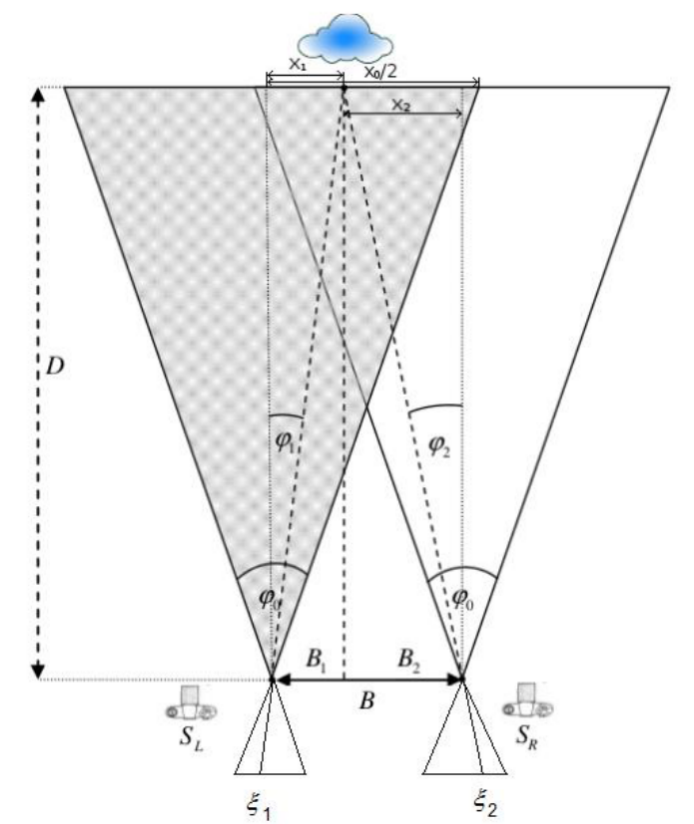
\includegraphics[width=0.6\textwidth]{figs/geom_model}
\caption{Geometric model of the stereo pair. Two cameras with parallel optical axes pointing to zenith observe a cloud at height $D$. The disparity $|\xi_1 - \xi_2|$ is inversely proportional to height.}
\label{fig:geom}
\end{figure}

\subsection{Affine calibration by solar position}

Equation~(\ref{eq:height}) requires strictly parallel optical axes, which is practically unattainable in field conditions due to mutual rotation and displacement of the cameras. We address this by computing an affine transformation $H \in \mathbb{R}^{3 \times 3}$ that rectifies the images to a common coordinate frame:
\begin{equation}
H = \begin{pmatrix} r_1 & r_2 & t_1 \\ r_3 & r_4 & t_2 \\ 0 & 0 & 1 \end{pmatrix},
\end{equation}
where the $2 \times 2$ submatrix encodes rotation and the vector $(t_1, t_2)^\top$ encodes translation. Calibration is performed using the Sun as an infinitely distant reference object: when optical axes are perfectly aligned, the Sun projects to identical pixel coordinates in both views.

Given $K \ge 3$ pairs of corresponding solar positions $(x_1^{(i)}, y_1^{(i)})$ on image~\#1 and $(x_2^{(i)}, y_2^{(i)})$ on image~\#2, the matrix $H$ is estimated by minimising the reprojection error:
\begin{equation}
\sum_{i=1}^{K} \left\| \begin{pmatrix} x_1^{(i)} \\ y_1^{(i)} \\ 1 \end{pmatrix} - H \begin{pmatrix} x_2^{(i)} \\ y_2^{(i)} \\ 1 \end{pmatrix} \right\|^2 \to \min.
\end{equation}
In practice, $H$ is computed using OpenCV's \texttt{estimateAffine2D} with RANSAC initialisation. Image~\#1 is warped by $H$ to produce image~\#1$'$; feature matching is then performed between \#1$'$ and the original image~\#2. This order of operations---applying the affine transformation before matching---eliminates the need for a separate coordinate transformation stage.

For the system deployed in this study, calibration performed on May~29, 2023 yielded a rotation submatrix close to identity, confirming near-parallel physical alignment of the cameras~\cite{3,4}. However, calibration stability is limited: diurnal temperature variations and wind-induced mechanical deformations can cause the effective affine parameters to drift. Repeat calibrations on different days revealed disparity shifts of up to 30 pixels for the same object, equivalent to $\approx 900$~m in height, motivating regular recalibration before each observation session.

\section{Feature Matching and Clustering}\label{sec:matching}

\subsection{LoFTR: detector-free dense matching}

Traditional feature matching pipelines (SIFT, ORB, SuperPoint) follow a detect-then-describe paradigm: keypoints are first detected, then matched across views. Cloud images present a particularly challenging scenario for this approach: their semi-transparent, diffuse texture yields few reliable keypoints with classical detectors, and the repetitive patterns of cloud formations lead to ambiguous descriptors. Furthermore, matching in homogeneous regions (clear sky) produces false correspondences that survive ratio-test filtering.

We employ LoFTR (Local Feature TRansformer)~\cite{1}, a detector-free architecture that directly produces dense correspondences from an image pair without a separate keypoint detection stage. LoFTR uses a Vision Transformer (ViT) backbone~\cite{5}: each image is divided into patches, which are encoded into embeddings by a convolutional neural network. Self-attention layers model long-range dependencies within each image, while cross-attention layers establish correspondences between the two views. Unlike convolutional backbones with limited receptive fields, the global attention mechanism enables LoFTR to leverage contextual cues---such as large-scale cloud texture gradients and illumination patterns---that are invisible to local detectors.

The output is a set of several hundred to over a thousand sub-pixel correspondences per frame, dramatically denser than what classical keypoint methods provide. Each correspondence yields a disparity vector $\Delta\vec{r} = (\Delta\xi, \Delta\eta)$; Eq.~(\ref{eq:height}) uses only the horizontal component $\Delta\xi$, while the vertical component $\Delta\eta$ should approach zero after affine rectification, providing a useful quality check. Figure~\ref{fig:localization} shows the spatial distribution of LoFTR matches on the original images, colour-coded by their subsequent HDBSCAN cluster assignments.

\begin{figure}[t]
\centering
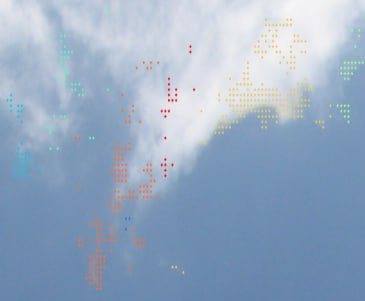
\includegraphics[width=0.72\textwidth]{figs/localization_crop}
\caption{Spatial localisation of LoFTR correspondences on the original stereo image pair. Points are colour-coded by their HDBSCAN cluster assignment, illustrating that clusters in disparity space correspond to spatially coherent regions of the cloud field.}
\label{fig:localization}
\end{figure}

\subsection{HDBSCAN clustering in disparity space}

Not all LoFTR correspondences are physically meaningful: some arise from clear-sky regions, lens artefacts, or sensor noise. In conditions of multi-layered cloudiness, correspondences belong to different cloud layers at distinct heights, producing multiple modes in the disparity distribution. To separate valid correspondences from outliers and to resolve multiple cloud layers, we apply HDBSCAN (Hierarchical Density-Based Spatial Clustering of Applications with Noise)~\cite{2} in the 2D disparity space $(\Delta\xi, \Delta\eta)$.

HDBSCAN offers several advantages over traditional clustering algorithms for this task: it requires no a priori specification of the number of clusters, it automatically identifies noise points without arbitrary density thresholds, and its hierarchical nature allows it to find clusters of varying density---an important property when cloud layers at different heights produce disparity clusters with different spreads. Each resulting cluster corresponds to a distinct cloud layer; the cluster centroid disparity is converted to a height estimate via Eq.~(\ref{eq:height}), and the spread of disparities within the cluster provides a natural uncertainty measure. The primary CBH estimate for each frame is taken as the height of the lowest reliable cluster, reflecting the meteorological definition of cloud base.

\begin{figure}[t]
\centering
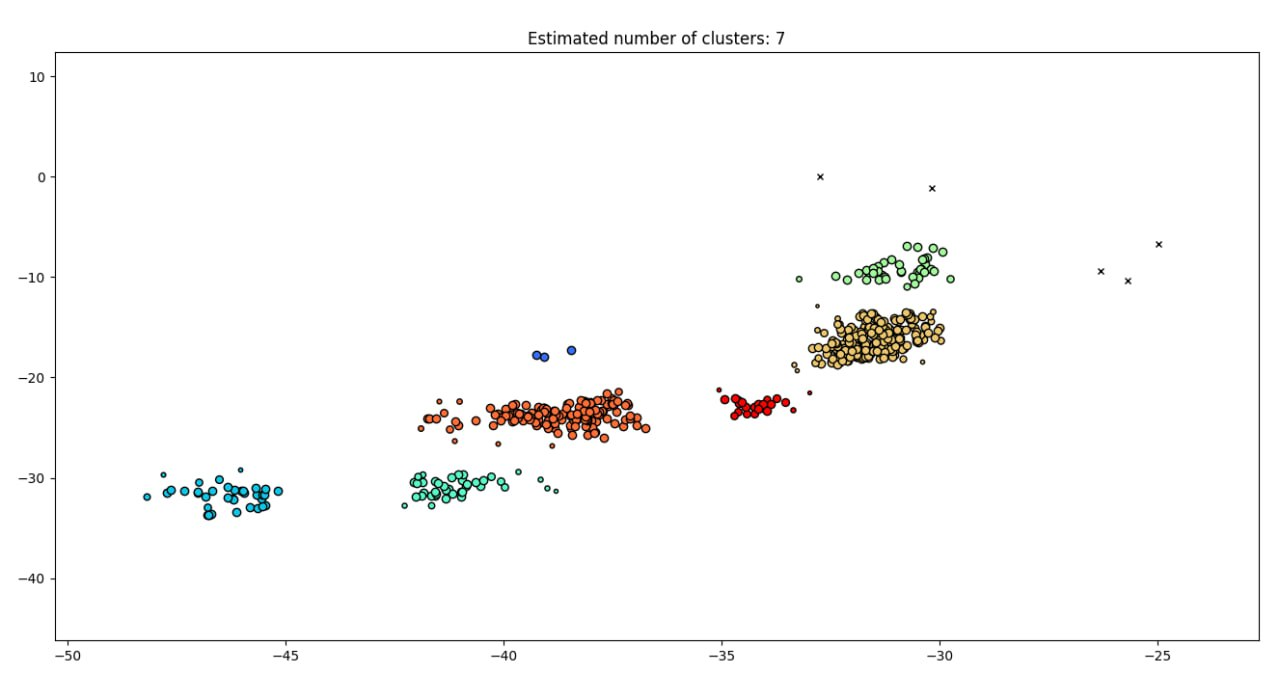
\includegraphics[width=0.80\textwidth]{figs/cluster}\\[4pt]
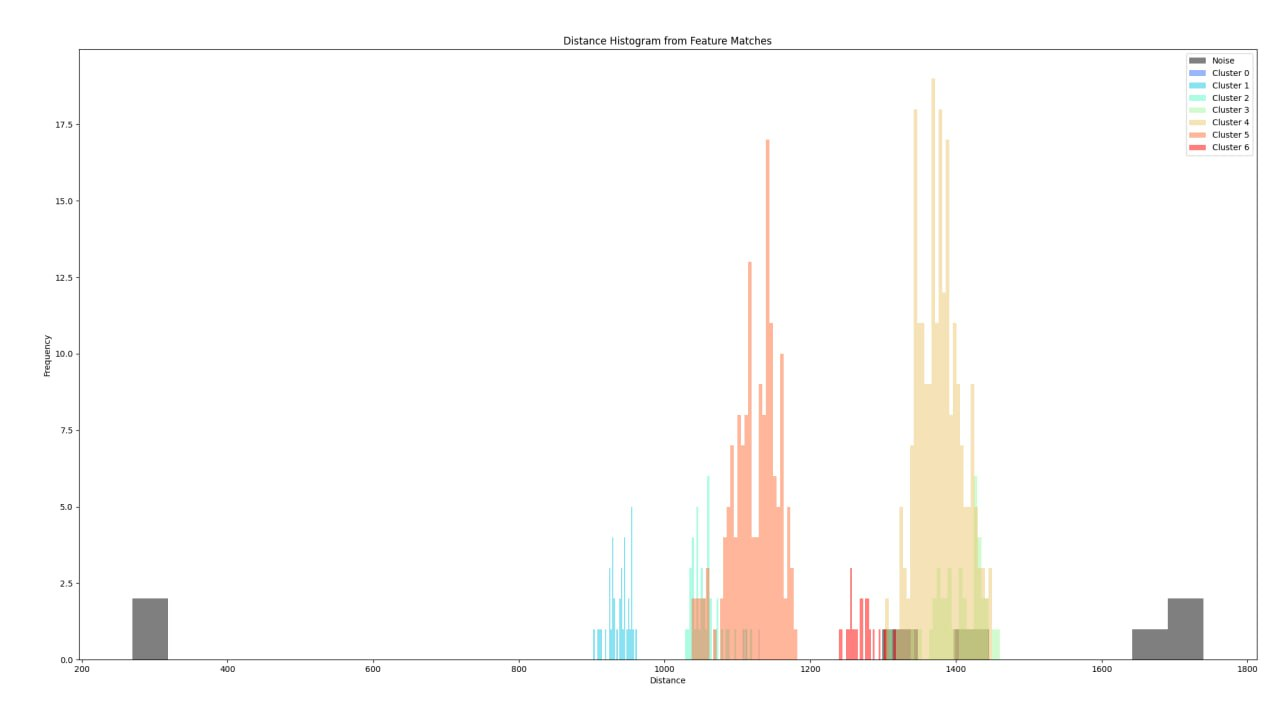
\includegraphics[width=0.80\textwidth]{figs/height_dist}
\caption{HDBSCAN clustering of LoFTR correspondences in 2D disparity space $(\Delta\xi, \Delta\eta)$ (top) and the derived height distribution per cluster (bottom). Ceilometer reference: 1300~m.}
\label{fig:cluster}
\end{figure}

\section{Spatial Filtering of Clusters}\label{sec:spatial}

HDBSCAN clusters points by proximity in disparity space but does not verify whether the corresponding image points form a physically connected region in the image plane. This can lead to two types of artefacts: (i)~two spatially distant cloud patches at the same height can produce identical disparities and be merged into a single cluster, even though they belong to physically independent cloud fields; (ii)~spurious LoFTR matches in clear-sky regions or near lens artefacts may survive HDBSCAN and form parasitic clusters with plausible disparity statistics. To address these issues, we apply a three-stage spatial filter to each cluster before it enters the temporal tracker.

\subsection{Stage 1: DBSCAN sub-clustering in image space}

For each HDBSCAN cluster, DBSCAN is run on keypoint coordinates in the first image ($\varepsilon = 30$~px, $\text{min\_samples} = 3$). Only the largest spatial sub-cluster is retained; noise points and minor sub-clusters are discarded. Clusters falling below a point-count threshold are rejected, eliminating cases where HDBSCAN merges spatially unrelated cloud patches.

\subsection{Stage 2: Convex-hull density check}

A convex hull is built around surviving points, and the density $\rho = n_\text{pts} / \text{area}$ is computed. Clusters with $\rho < 0.002$~pts/px$^2$ are rejected: sparse scatter at similar disparity cannot correspond to a continuous cloud surface.

\subsection{Stage 3: Neighbour-consistency verification}

For each point, the $K = 5$ nearest neighbours in image space are found. If the fraction of points whose neighbourhood disparity deviation exceeds $2.0 \cdot \sigma_\text{disp}$ surpasses 30\%, the cluster is rejected. This enforces the property that image-space proximity implies disparity similarity for continuous 3D surfaces.

In aggregate, the three-stage spatial filter eliminates 15--25\% of candidate clusters. The computational overhead is negligible relative to the LoFTR inference cost, and the improvement in tracker input purity directly translates to more stable Kalman filter operation.

\section{Adaptive Kalman Filter for Temporal Consistency}\label{sec:kalman}

\subsection{Problem formulation}

Without temporal processing, each stereo pair is analysed independently, yielding physically unrealistic jumps (up to 500~m per 10~s), cluster fragmentation across frames, and low autocorrelation ($r_\text{auto} \approx 0.11$ over 5~hours). We model cloud height evolution as uniform motion:
\begin{equation}
h_{t+1} = h_t + \dot{h}_t \Delta t, \qquad \dot{h}_{t+1} = \dot{h}_t,
\end{equation}
with state vector $\mathbf{x}_t = [h_t, \dot{h}_t]^\top$ and transition matrix
\begin{equation}
\mathbf{F} = \begin{pmatrix} 1 & \Delta t \\ 0 & 1 \end{pmatrix}.
\end{equation}
The process noise covariance $\mathbf{Q}$ is parameterised by the vertical acceleration uncertainty $\sigma_h = 5.0$~m/s$^2$:
\begin{equation}
\mathbf{Q} = \sigma_h^2 \begin{pmatrix} \Delta t^4/4 & \Delta t^3/2 \\ \Delta t^3/2 & \Delta t^2 \end{pmatrix}.
\end{equation}
This parameterisation corresponds to a random-walk acceleration model (piecewise-constant Wiener process acceleration), reflecting the physical expectation that cloud height changes are driven by smooth atmospheric processes rather than discontinuous jumps.

Before filtering, clusters differing in height by less than 300~m are merged to counteract HDBSCAN-induced fragmentation of single cloud layers. Three strategies are available for selecting the target cluster: \texttt{largest} (maximum point count), \texttt{lowest} (meteorological cloud base), and \texttt{lowest\_reliable} (lowest with point count above a threshold).

\subsection{Innovation-adaptive measurement covariance}

A fixed measurement noise covariance $R$ is fundamentally unsuitable for this task: it cannot simultaneously track genuine height variations (requiring small $R$ to respond quickly) and reject outliers (requiring large $R$ to ignore spurious measurements). We adopt an innovation-adaptive scheme where $R$ scales with the squared deviation of the current measurement from the Kalman prediction:
\begin{equation}
R = \text{clip}\left(R_\text{scale} \cdot \max(|z - \hat{x}^-|, 10)^2 \cdot 0.01,\; 100,\; 10^6\right),
\label{eq:adaptive}
\end{equation}
with $R_\text{scale} = 50$. The clipping bounds $[100, 10^6]$ prevent degenerate behaviour. At small innovations the filter trusts the measurement; at large innovations it relies on prediction, automatically suppressing outliers without hard thresholds. Measurement uncertainty uses SEM: $\sigma_h^{\text{SEM}} = f(\sigma_\text{disp} / \sqrt{n_\text{pts}})$, yielding $\sigma_h^{\text{SEM}} \approx 5$~m for a typical 566-point cluster vs.\ $\sigma_h^{\text{std}} \approx 124$~m---a 25-fold reduction critical for correct Kalman gain balancing.

\section{Experimental Results}\label{sec:results}

\subsection{Data acquisition and preprocessing}

The stereo system consists of two fisheye cameras ($\phi_0 = 180^\circ$, $1920 \times 1080$~px) on a 45~m baseline, both pointing to zenith, acquiring images every 10~s. A central $640 \times 640$~px crop was used for analysis. Ground truth was provided by a co-located DOL-2 laser ceilometer (10--3000~m range, $\pm(5 + 0.05H)$~m accuracy)~\cite{6}.

The primary validation dataset consists of a 5-hour sequence (12:00--17:00 MSK) acquired on May~23, 2025, covering conditions from homogeneous stratus to broken multi-layer cumulus with varying wind directions. For each stereo pair, the processing chain proceeds as follows: affine rectification, LoFTR dense matching, HDBSCAN clustering, spatial filtering, and conversion of the lowest cluster's centroid disparity to height via Eq.~(\ref{eq:height}).

\subsection{Kalman filter performance}

Table~\ref{tab:kalman} summarises the effect of the adaptive Kalman filter on key metrics of the CBH time series.

\begin{table}[t]
\centering
\caption{Comparison of cloud base height time-series metrics before and after application of the adaptive Kalman filter. All metrics are computed over the 5-hour validation sequence (May~23, 2025).}\label{tab:kalman}
\begin{tabular}{lccc}
\hline
Metric & Raw estimates & Kalman-filtered & Improvement \\
\hline
Mean frame-to-frame jump $|\Delta h|$ (10~s) & 515~m & 120~m & $\mathbf{\times 4.3}$ \\
5-hour autocorrelation ($\tau = 10$~s) & 0.11 & 0.90 & $\mathbf{\times 8.0}$ \\
Mean $r$ in 30-min windows & 0.55 & 0.67 & $+22\%$ \\
Fraction of windows with $r > 0.5$ & 61\% (11/18) & 72\% (13/18) & --- \\
Maximum $r$ in a single window & 0.88 & 0.94 & --- \\
\hline
\end{tabular}
\end{table}

The filter reduces the median frame-to-frame height jump by a factor of 4.3 (from 515~m to 120~m) and raises the 5-hour autocorrelation from 0.11 to 0.90, transforming a physically incoherent sequence into a smooth trajectory. The mean correlation with the ceilometer increases from $r = 0.55$ to $r = 0.67$, and the fraction of windows exceeding $r = 0.5$ rises from 61\% to 72\%.

\subsection{Windowed correlation with dynamic time-shift alignment}

Wind-driven cloud advection causes a variable temporal lag between the instruments. To account for this, the series is split into 30-minute windows with individual time-shift alignment maximising cross-correlation. The global 5-hour raw correlation between stereo estimates and the ceilometer is $r \approx 0.04$; after windowed dynamic alignment, the mean per-window correlation reaches $r = 0.67$, with 72\% of windows exceeding $r = 0.5$ and a maximum of $r = 0.94$ under homogeneous cloud cover.

\begin{figure}[t]
\centering
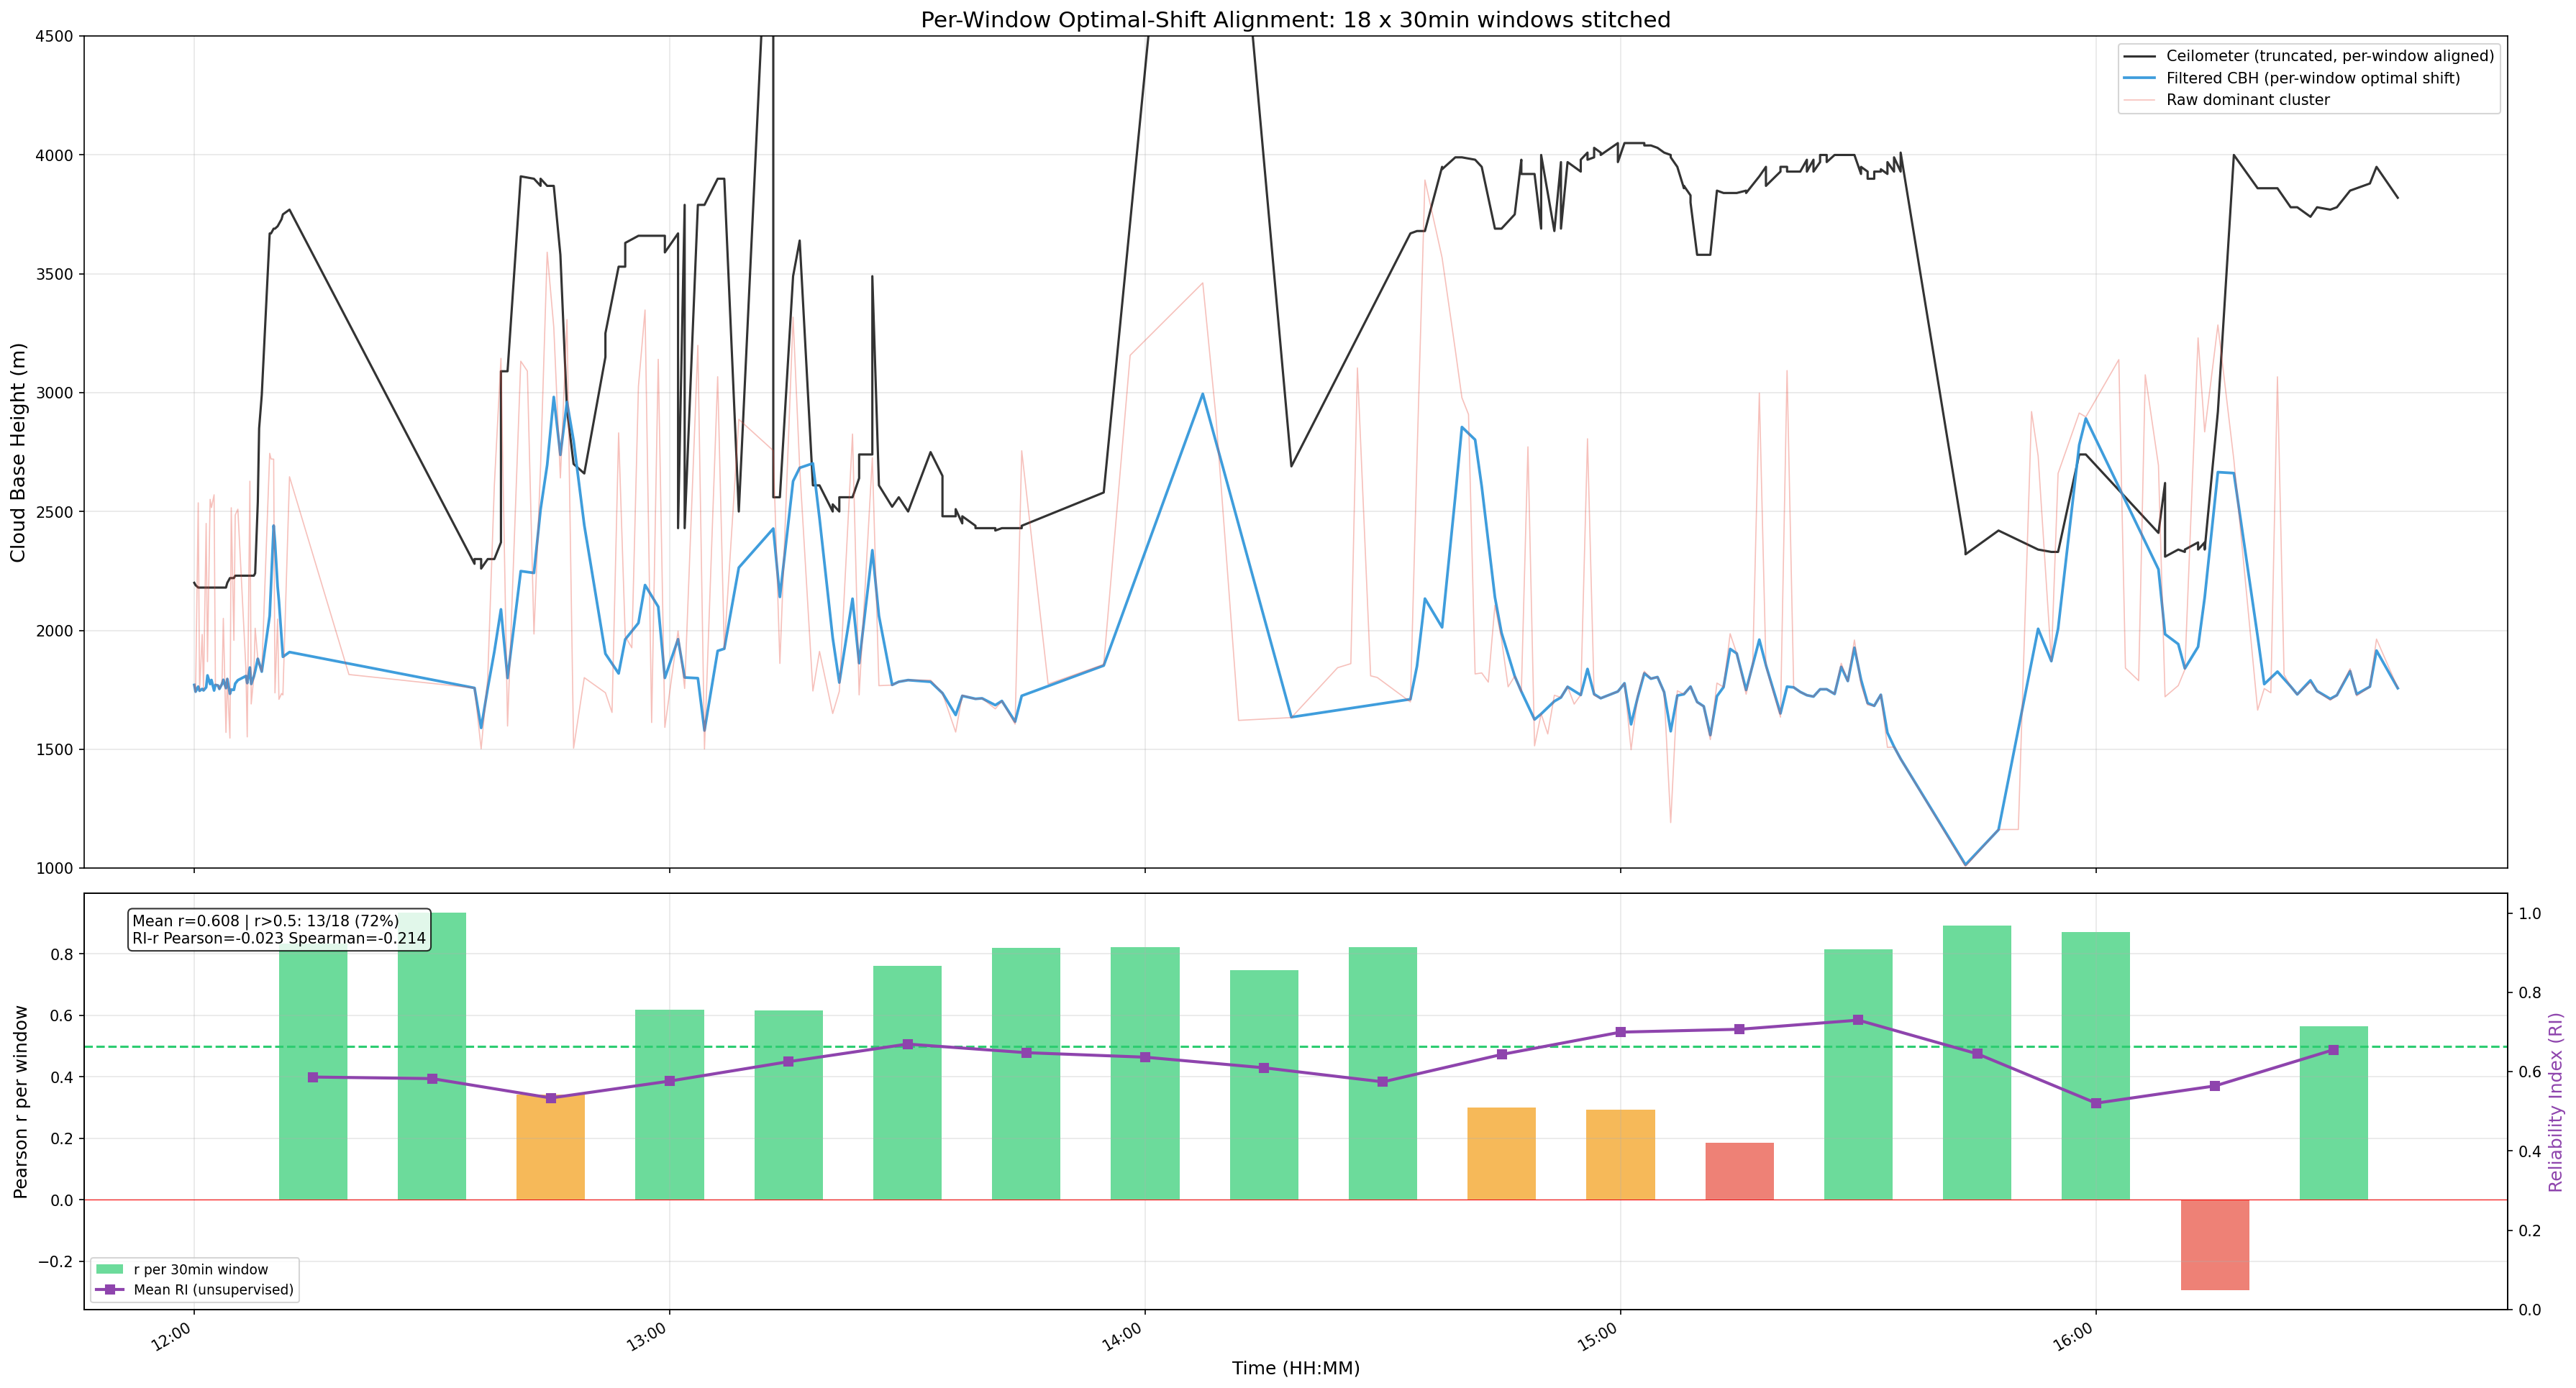
\includegraphics[width=0.95\textwidth]{figs/01_stitched_windows}
\caption{Stitched time series of cloud base height over the 5-hour validation period (May~23, 2025). \textbf{Top panel:} height time series for the ceilometer (red), raw per-frame stereo estimates (green), and Kalman-filtered stereo estimates (blue). The vertical offset between ceilometer and stereo traces is discussed in Section~\ref{sec:bias}. \textbf{Bottom panel:} Pearson correlation coefficient $r$ between the stereo pipeline and the ceilometer in each 30-minute window (orange). Windows with $r > 0.5$ correspond to homogeneous cloud cover; lower correlations occur during transitions and multi-layer conditions.}
\label{fig:stitched}
\end{figure}

The per-window correlation pattern in Fig.~\ref{fig:stitched} (bottom) reveals that windows with $r < 0.5$ correspond to periods of multi-layer cloudiness, rapid wind direction changes, or transitions between cloud regimes---conditions where the assumption of a single dominant cloud layer per window is violated. The highest correlations ($r = 0.88$--0.94) occur under homogeneous stratus or well-defined single cumulus decks.

\subsection{Cluster merge and selection}

Prior to filtering, clusters with height differences below 300~m are merged to counteract HDBSCAN-induced fragmentation. The \texttt{lowest} selection strategy (meteorological cloud base) provides the most consistent results for ceilometer comparison, yielding mean $r = 0.55$ (raw) and $r = 0.67$ (filtered) vs.\ $r = 0.51/0.56$ for the \texttt{largest} strategy. This is expected, as the ceilometer also reports the lowest detected layer.

\section{Systematic Bias of the Laser Ceilometer}\label{sec:bias}

A persistent vertical offset (Fig.~\ref{fig:stitched}) stems from different measurement principles. The DOL-2 ceilometer detects the backscattered laser signal exceeding a threshold \emph{inside} the cloud layer~\cite{6}, measuring an \textbf{optical} base. The stereo system measures the \textbf{geometric} boundary via scattered sunlight. The offset magnitude---always non-negative (ceilometer $\ge$ stereo)---varies with cloud type and droplet distribution, consistent with the observed diurnal variation of the vertical shift in Fig.~\ref{fig:stitched}.

\section{Conclusions}\label{sec:conclusions}

We have presented a complete pipeline for cloud base height estimation from ground-based stereo fisheye images, combining LoFTR-based dense feature matching with HDBSCAN clustering, three-stage spatial filtering, and innovation-adaptive Kalman filtering. The main findings are:

\begin{enumerate}
\item \textbf{LoFTR provides robust dense correspondences} in texture-poor cloud images where traditional keypoint detectors fail.

\item \textbf{HDBSCAN clustering} separates distinct cloud layers and rejects outliers without prior specification of the cluster count. The three-stage spatial filter eliminates 15--25\% of implausible clusters.

\item \textbf{The adaptive Kalman filter} reduces frame-to-frame height jumps by a factor of~4.3 and increases the 5-hour autocorrelation from~0.11 to~0.90, transforming a physically incoherent sequence into a smooth trajectory with automatic outlier suppression.

\item \textbf{After windowed dynamic time-shift alignment}, the pipeline achieves a mean $r = 0.67$ with a ceilometer, with 72\% of 30-minute windows exceeding $r = 0.5$ ($\max r = 0.94$).

\item \textbf{The systematic offset} between stereo and ceilometer data is explained by the difference between geometric and optical CBH measurement, establishing stereo vision as a complementary modality.
\end{enumerate}

Limitations include calibration drift and inability to operate under featureless overcast. Future work will address online recalibration and distributed low-cost CBH monitoring.

\begin{acknowledgments}
The authors thank the staff of the Meteorological Observatory of M.V. Lomonosov Moscow State University for providing ceilometer data and for maintaining the stereo camera installation.
\end{acknowledgments}

\section*{FUNDING}
This work was supported by the M.V. Lomonosov Moscow State University research program.

\section*{CONFLICT OF INTEREST}
The authors of this work declare that they have no conflicts of interest.

\begin{thebibliography}{}

\bibitem{1}
J. Sun, Z. Shen, Y. Wang, H. Bao, and X. Zhou,
``LoFTR: Detector-Free Local Feature Matching with Transformers,''
in \emph{Proc. IEEE/CVF Conf. Computer Vision and Pattern Recognition (CVPR)},
2021, pp. 8922--8931.
https://doi.org/10.1109/CVPR46437.2021.00881

\bibitem{2}
R. J. G. B. Campello, D. Moulavi, and J. Sander,
``Density-Based Clustering Based on Hierarchical Density Estimates,''
in \emph{Advances in Knowledge Discovery and Data Mining (PAKDD)},
Lect. Notes Comput. Sci., vol. 7819, Springer, 2013, pp. 160--172.
https://doi.org/10.1007/978-3-642-37456-2\_14

\bibitem{3}
S. V. Nikitin and A. I. Chulichkov,
``Mathematical modelling of a cloud image analysis system for estimating cloud height and velocity,''
Moscow, 2018. (In Russian).

\bibitem{4}
M. S. Andreev and A. I. Chulichkov,
``Computer methods for estimating cloud height and velocity from their images,''
Moscow, 2014. (In Russian).

\bibitem{5}
A. Dosovitskiy et al.,
``An Image is Worth 16x16 Words: Transformers for Image Recognition at Scale,''
in \emph{Proc. Int. Conf. Learning Representations (ICLR)}, 2021.

\bibitem{6}
Laser cloud sensor DOL-2. Technical description.
LOMO METE LLC, Planeta Info LLC.
\url{https://oplanete.info}. (In Russian).

\end{thebibliography}
\end{document}
